% ======================================================================
%  Appendix B — Differential Forms and Chern Classes  (EXPANDED)
% ======================================================================

\section{Motivation: why differential forms?}
\label{sec:appB-motivation}

The Berry connection, Berry curvature, and Chern number are most
naturally expressed in the language of differential forms on the
Brillouin zone \cite{atala2013direct}.  While the coordinate-based formulas used in the main
text are sufficient for computation, the differential-form viewpoint
clarifies \emph{why} the Chern number is an integer, why it is
gauge-invariant, and how it generalises to higher dimensions and
non-Abelian bundles.

This appendix provides a self-contained introduction to the relevant
mathematics.  The reader who is comfortable with exterior calculus can
skip to \secref{sec:appB-chern-class}; the reader who wants only the
practical formulas can use the summary table at the end.

\section{Differential forms on the Brillouin zone}
\label{sec:appB-forms}

\subsection{The Brillouin zone as a manifold}
\label{sec:appB-bz-manifold}

The first Brillouin zone (BZ) of a 2D lattice is a parallelogram in
reciprocal space with opposite edges identified.  Topologically, it is
a 2-torus $T^2=S^1\times S^1$.  For a 3D lattice, $\BZ\cong T^3$.

A differential $p$-form on $T^d$ is a smooth antisymmetric tensor
field of rank $p$.  In coordinates $(k_1,\ldots,k_d)$:
\begin{equation}\label{eq:appB-p-form}
  \alpha = \sum_{i_1<\cdots<i_p}
  \alpha_{i_1\cdots i_p}(\kvec)\,
  \dd k_{i_1}\wedge\cdots\wedge\dd k_{i_p}\,.
\end{equation}

\subsection{The exterior derivative}
\label{sec:appB-exterior-d}

The exterior derivative $\dd$ maps $p$-forms to $(p+1)$-forms:
\begin{equation}\label{eq:appB-exterior-d}
  \dd\alpha = \sum_j\pderiv{\alpha_{i_1\cdots i_p}}{k_j}\,
  \dd k_j\wedge\dd k_{i_1}\wedge\cdots\wedge\dd k_{i_p}\,.
\end{equation}
The key property is $\dd^2=0$, which is the form-language version of
$\nabla\times(\nabla\phi)=0$ and $\nabla\cdot(\nabla\times\mathbf{F})=0$.

\subsection{Integration of forms}
\label{sec:appB-integration}

A $p$-form can be integrated over a $p$-dimensional oriented manifold:
\begin{equation}\label{eq:appB-integration}
  \int_{T^2}\Omega = \int_\BZ\Omega_{12}(\kvec)\,
  \dd k_1\wedge\dd k_2\,.
\end{equation}
Stokes' theorem in form language is $\int_M\dd\alpha
=\oint_{\partial M}\alpha$.  Since $T^2$ has no boundary
($\partial T^2=\emptyset$), $\int_{T^2}\dd\alpha=0$ for any 1-form
$\alpha$.

\section{The Bloch bundle}
\label{sec:appB-bundle}

\subsection{Definition}
\label{sec:appB-bundle-def}

At each $\kvec\in\BZ$, the Maxwell eigenvalue problem produces a set of
eigenmodes $|\mathbf{u}_{n\kvec}\rangle$.  Fixing a band $n$, the
collection of one-dimensional subspaces
$\{|\mathbf{u}_{n\kvec}\rangle\}_{\kvec\in\BZ}$ forms a complex line
bundle over the torus $T^2$.  This is the \emph{Bloch bundle} of band
$n$.

More precisely, the Bloch bundle is the fibre bundle
$\pi:E_n\to T^2$ with fibre $\mathbb{C}$ and structure group $U(1)$
\cite{raghu2008analogs,nakahara2018geometry,sergeev2018geometry}.
A \emph{section} of this bundle is a smooth assignment
$\kvec\mapsto|\mathbf{u}_{n\kvec}\rangle$ (i.e., a smooth gauge
choice).

Figure~\ref{fig:appB-bloch-bundle-forms} translates this definition
into the geometric picture used in the main text.  The Brillouin zone
is a torus, not an open square: opposite edges are identified.  Above
each point of this torus sits the one-dimensional eigenspace of the
chosen Maxwell band.  A local Berry connection records how a normalised
mode changes along a path in $\kvec$-space, while the curvature
measures the infinitesimal rotation accumulated around a small area.
The first Chern number is the total curvature flux through this torus.

\begin{figure}[t]
  \centering
  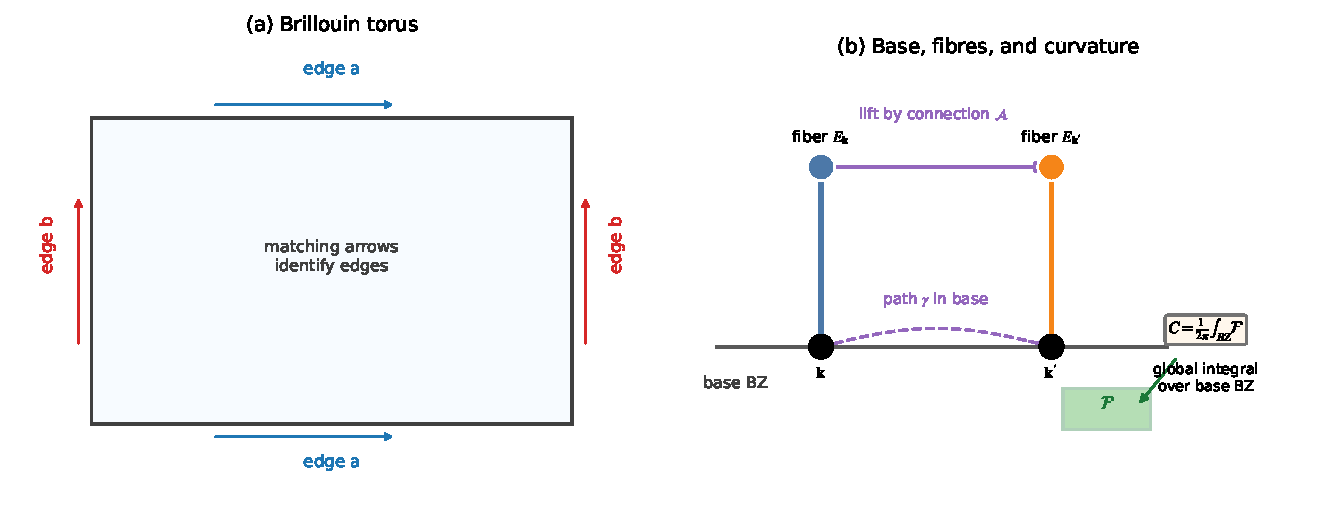
\includegraphics[width=0.88\textwidth]{figures/fig_appB_bloch_bundle_forms.pdf}
  \caption{The Bloch bundle and Berry curvature in differential-form
  language.  The base space is the Brillouin-zone torus $T^2$, drawn as
  a fundamental square with opposite sides identified.  Fibres are the
  Maxwell eigenspaces of a chosen band, the Berry connection
  $\mathcal{A}$ transports phases along paths, and the curvature
  $\mathcal{F}=\dd\mathcal{A}$ is an oriented two-form.  The Chern
  number is the total curvature flux, $C=(2\pi)^{-1}\int_{T^2}
  \mathcal{F}$.}
  \label{fig:appB-bloch-bundle-forms}
\end{figure}


\subsection{Gauge transformations}
\label{sec:appB-gauge}

A gauge transformation is a smooth map $g:T^2\to U(1)$,
$\kvec\mapsto\ee^{\ii\chi(\kvec)}$, which acts on sections by
$|\mathbf{u}_{n\kvec}\rangle\mapsto\ee^{\ii\chi(\kvec)}
|\mathbf{u}_{n\kvec}\rangle$.

Not every line bundle admits a globally smooth section.  A bundle that
does is called \emph{trivial}; one that does not is \emph{nontrivial}.
The Chern number measures the obstruction to triviality.

\section{Connection and curvature}
\label{sec:appB-connection}

\subsection{The Berry connection as a 1-form}
\label{sec:appB-berry-1form}

The Berry connection of band $n$ is the $U(1)$ connection 1-form on the
Bloch bundle:
\begin{equation}\label{eq:appB-berry-connection}
  \mathcal{A}_n
  = \ii\langle\mathbf{u}_{n\kvec}|\Mgmat|\dd\mathbf{u}_{n\kvec}\rangle
  = \sum_a\Aberry_{n,a}(\kvec)\,\dd k_a\,,
\end{equation}
where $\dd\mathbf{u}_{n\kvec}=\sum_a(\partial_{k_a}\mathbf{u}_{n\kvec})
\dd k_a$ and the inner product uses the electromagnetic energy metric
$\Mgmat$.

Under a gauge transformation $|\mathbf{u}\rangle\to\ee^{\ii\chi}
|\mathbf{u}\rangle$:
\begin{equation}\label{eq:appB-gauge-transform}
  \mathcal{A}_n\to\mathcal{A}_n-\dd\chi\,.
\end{equation}
This is the electromagnetic analog of the $U(1)$ gauge transformation
in electrodynamics.

\subsection{The Berry curvature as a 2-form}
\label{sec:appB-berry-2form}

The Berry curvature is the curvature 2-form of the connection:
\begin{equation}\label{eq:appB-berry-curvature}
  \mathcal{F}_n = \dd\mathcal{A}_n
  = \Omega_n(\kvec)\,\dd k_1\wedge\dd k_2\,,
\end{equation}
where $\Omega_n=\partial_{k_1}\Aberry_{n,2}
-\partial_{k_2}\Aberry_{n,1}$ is the Berry curvature scalar in 2D.

The curvature is gauge-invariant: under $\mathcal{A}_n\to
\mathcal{A}_n-\dd\chi$, we have $\mathcal{F}_n\to\dd\mathcal{A}_n
-\dd^2\chi=\mathcal{F}_n$ (using $\dd^2=0$).

\section{The first Chern class and integrality} \cite{kane2005sub}
\label{sec:appB-chern-class}

\subsection{Definition}
\label{sec:appB-chern-def}

The first Chern number of the Bloch bundle is
\begin{equation}\label{eq:appB-chern}
  \boxed{%
  \Chern_n = \frac{1}{2\pi}\int_{T^2}\mathcal{F}_n
  = \frac{1}{2\pi}\int_\BZ\Omega_n(\kvec)\,\dd^2k\,.}
\end{equation}

\subsection{Proof of integrality}
\label{sec:appB-integrality}

The Chern number is always an integer.  The proof uses the
patchwise construction of the bundle.

Cover $T^2$ with two open sets $U_N$ and $U_S$ (``north'' and
``south'' patches, each a disc) such that $U_N\cup U_S=T^2$ and the
overlap $U_N\cap U_S\cong S^1$ is an annulus.

On each patch, choose a smooth gauge and compute the Berry connection:
$\mathcal{A}_N$ on $U_N$, $\mathcal{A}_S$ on $U_S$.  On the overlap,
the two gauges are related by a transition function
$g_{NS}:U_N\cap U_S\to U(1)$, so
$\mathcal{A}_N=\mathcal{A}_S-\dd\chi_{NS}$.

By Stokes' theorem on each patch:
\begin{align}
  \int_{U_N}\mathcal{F}_N &= \oint_{\partial U_N}\mathcal{A}_N\,,\\
  \int_{U_S}\mathcal{F}_S &= -\oint_{\partial U_S}\mathcal{A}_S\,,
\end{align}
where the signs reflect orientation.  Adding:
\begin{align}
  \int_{T^2}\mathcal{F}
  &= \oint_{\partial U_N}\mathcal{A}_N
  + \oint_{\partial U_S}\mathcal{A}_S
  \notag\\
  &= \oint_{S^1}(\mathcal{A}_N-\mathcal{A}_S)
  = -\oint_{S^1}\dd\chi_{NS}
  \notag\\
  &= -[\chi_{NS}]_{S^1}\,.
\end{align}
The transition function $g_{NS}=\ee^{\ii\chi_{NS}}$ must be
single-valued on $S^1$, so $[\chi_{NS}]_{S^1}=2\pi\nu$ for some
integer $\nu$.  Therefore $\Chern_n=\nu\in\mathbb{Z}$.

This proof shows that the Chern number counts the winding number of
the transition function around the overlap circle---equivalently, the
number of times the gauge must ``twist'' as the momentum traverses the
Brillouin zone.

\subsection{Physical interpretation}
\label{sec:appB-physical}

A nonzero Chern number means the Bloch bundle is nontrivial: there is
no globally smooth gauge choice for the cell-periodic modes over the
entire Brillouin zone.  This obstruction is precisely what forces the
existence of edge modes at the boundary of the material, through the
bulk-edge correspondence.

\section{Non-Abelian generalisation}
\label{sec:appB-non-abelian}

\subsection{Multi-band bundles}
\label{sec:appB-multi-band}

When $p$ bands are degenerate or nearly degenerate, they form a
rank-$p$ vector bundle with structure group $U(p)$.  The Berry
connection becomes a matrix-valued 1-form:
\begin{equation}\label{eq:appB-na-connection}
  [\mathcal{A}]_{\alpha\beta}
  = \ii\langle\mathbf{u}_{\alpha\kvec}|\Mgmat|
  \dd\mathbf{u}_{\beta\kvec}\rangle\,,
  \qquad \alpha,\beta=1,\ldots,p\,.
\end{equation}
The curvature is
\begin{equation}\label{eq:appB-na-curvature}
  \mathcal{F} = \dd\mathcal{A}+\mathcal{A}\wedge\mathcal{A}\,.
\end{equation}
The non-Abelian Berry curvature has the extra quadratic term
$\mathcal{A}\wedge\mathcal{A}$, which vanishes in the Abelian
($p=1$) case.

\subsection{The non-Abelian Chern number}
\label{sec:appB-na-chern}

The first Chern number of the rank-$p$ bundle is
\begin{equation}\label{eq:appB-na-chern-formula}
  \Chern = \frac{1}{2\pi}\int_{T^2}\Tr(\mathcal{F})\,.
\end{equation}
Note that only the \emph{trace} of the curvature enters.  This is
gauge-invariant (invariant under $U(p)$ gauge transformations) and is
always an integer.

\subsection{The second Chern number}
\label{sec:appB-second-chern}

In four dimensions, the second Chern number is
\begin{equation}\label{eq:appB-second-chern}
  \Chern_2 = \frac{1}{8\pi^2}\int_{T^4}
  \Tr(\mathcal{F}\wedge\mathcal{F})\,.
\end{equation}
This is a topological invariant of bundles over the 4-torus $T^4$
and appears in the theory of the 4D quantum Hall effect
(Chapter~\ref{ch:synthetic-dimensions}).

\section{Summary of correspondence}
\label{sec:appB-summary}

\begin{center}
\begin{tabular}{ll}
  \toprule
  \textbf{Photonic concept} & \textbf{Mathematical object} \\
  \midrule
  Brillouin zone & Torus $T^d$ \\
  Band eigenmodes $|\mathbf{u}_{n\kvec}\rangle$ &
    Section of line bundle $E_n$ \\
  Gauge choice & Trivialisation of $E_n$ \\
  Berry connection $\Aberry_n$ & $U(1)$ connection 1-form \\
  Berry curvature $\Omega_n$ & Curvature 2-form $\mathcal{F}_n$ \\
  Chern number $\Chern_n$ &
    First Chern class $c_1(E_n)\in\mathbb{Z}$ \\
  Multi-band connection & $U(p)$ connection \\
  Wilson loop & Holonomy of the connection \\
  Second Chern number &
    $c_2\in\mathbb{Z}$ (4D bundles) \\
  \bottomrule
\end{tabular}
\end{center}

The central message: the integrality of the Chern number is not a
numerical coincidence or an artefact of a particular computation
method.  It is a theorem of differential geometry, guaranteed by the
topology of the Brillouin-zone torus and the smoothness of the Bloch
bundle.  This is why the number of topological edge modes is exactly
quantised and robust to perturbations.

\section{The Hodge star and electromagnetic duality}
\label{sec:appB-hodge}

\subsection{Definition of the Hodge star}
\label{sec:appB-hodge-def}

On a $d$-dimensional oriented Riemannian manifold, the Hodge star
$\star$ is a linear map from $p$-forms to $(d-p)$-forms, defined by
the requirement that for any two $p$-forms $\alpha,\beta$:
\begin{equation}\label{eq:appB-hodge-def}
  \alpha\wedge\star\beta = \langle\alpha,\beta\rangle\,
  \mathrm{vol}\,,
\end{equation}
where $\langle\cdot,\cdot\rangle$ is the inner product induced by the
metric and $\mathrm{vol}$ is the volume form.

In three dimensions with Cartesian coordinates:
\begin{align}
  \star\dd x &= \dd y\wedge\dd z\,,\quad
  \star\dd y = \dd z\wedge\dd x\,,\quad
  \star\dd z = \dd x\wedge\dd y\,,\notag\\
  \star 1 &= \dd x\wedge\dd y\wedge\dd z\,,\quad
  \star(\dd x\wedge\dd y\wedge\dd z) = 1\,.
\end{align}
In particular, $\star\star\alpha=(-1)^{p(d-p)}\alpha$ for a $p$-form
in $d$ dimensions.  In three dimensions, $\star\star=+1$ on 1-forms
and 2-forms.

\subsection{Maxwell's equations in form language}
\label{sec:appB-maxwell-forms}

Maxwell's equations in vacuum can be written compactly using
differential forms.  Define the 2-forms $F$ (Faraday tensor) and
$\star F$ (its Hodge dual):
\begin{equation}\label{eq:appB-maxwell-forms}
  \dd F = 0\,,\qquad \dd\star F = \star J\,,
\end{equation}
where $J$ is the current 1-form.  The first equation encodes
$\nabla\times\Efield=-\partial_t\Bfield$ and $\nabla\cdot\Bfield=0$;
the second encodes $\nabla\times\Hfield=\Jfield+\partial_t\Dfield$
and $\nabla\cdot\Dfield=\rho$.  The electromagnetic duality
$F\to\star F$, $\star F\to -F$ is manifest in this language.

In a medium with material response, the constitutive relation
$\star F\mapsto\Mmat\,F$ replaces the vacuum Hodge star with the
material-weighted version, and the electromagnetic inner product of
Chapter~3 becomes the $L^2$ inner product with the material-modified
Hodge star as the metric.

\section{De Rham cohomology and topological obstructions}
\label{sec:appB-derham}

\subsection{Closed and exact forms}
\label{sec:appB-closed-exact}

A $p$-form $\alpha$ is \\emph{closed} if $\dd\alpha=0$ and
\\emph{exact} if $\alpha=\dd\beta$ for some $(p-1)$-form $\beta$.
Every exact form is closed (since $\dd^2=0$), but the converse is
not always true.  The quotient space
\begin{equation}\label{eq:appB-derham-cohomology}
  H^p_{\mathrm{dR}}(M) = \frac{\ker(\dd:
  \Lambda^p\to\Lambda^{p+1})}
  {\mathrm{im}(\dd:\Lambda^{p-1}\to\Lambda^p)}
\end{equation}
is the $p$-th de Rham cohomology group of the manifold $M$.  Its
dimension $b_p=\dim H^p_{\mathrm{dR}}(M)$ is the $p$-th Betti
number, a topological invariant of $M$.

For the 2-torus $T^2$: $b_0=1$ (connected), $b_1=2$ (two independent
non-contractible loops), $b_2=1$ (one independent ``area'' form).
The fact that $b_2=1$ means there exists exactly one independent
closed 2-form (modulo exact forms) on $T^2$.  The Berry curvature
$\mathcal{F}_n$ is a closed 2-form (since $\dd\mathcal{F}_n
=\dd^2\mathcal{A}_n=0$), and its cohomology class is characterised by
a single integer---the Chern number.

\subsection{The Poincar\'e lemma and its failure}
\label{sec:appB-poincare}

On a contractible domain (such as $\mathbb{R}^d$ or a disc), every
closed form is exact.  This is the Poincar\'e lemma: if
$\dd\alpha=0$, then $\alpha=\dd\beta$.  On the torus, the Poincar\'e
lemma \\emph{fails}: the Berry curvature $\mathcal{F}_n$ is closed but
not necessarily exact.  Its failure to be exact is precisely the
topological obstruction measured by the Chern number.  If $\Chern_n
\neq 0$, the Berry connection $\mathcal{A}_n$ cannot be defined
globally, and the Bloch bundle is nontrivial.

\section{The Chern--Simons 3-form} \cite{nittis2020equivalence}
\label{sec:appB-chern-simons}

\subsection{Definition}
\label{sec:appB-cs-def}

The Chern--Simons 3-form is defined for a connection 1-form
$\mathcal{A}$ with curvature $\mathcal{F}=\dd\mathcal{A}
+\mathcal{A}\wedge\mathcal{A}$ by
\begin{equation}\label{eq:appB-cs-form}
  \mathrm{CS}(\mathcal{A})
  = \mathcal{A}\wedge\dd\mathcal{A}
  + \tfrac{2}{3}\mathcal{A}\wedge\mathcal{A}\wedge\mathcal{A}\,.
\end{equation}
Its exterior derivative satisfies
$\dd\,\mathrm{CS}(\mathcal{A})=\Tr(\mathcal{F}\wedge\mathcal{F})$,
which is the integrand of the second Chern number.  In the Abelian
case ($U(1)$ bundle), $\mathcal{A}\wedge\mathcal{A}=0$ and
$\mathrm{CS}=\mathcal{A}\wedge\dd\mathcal{A}
=\mathcal{A}\wedge\mathcal{F}$.

\subsection{Role in topological photonics}
\label{sec:appB-cs-role}

The Chern--Simons form appears in several contexts in this book.
In three dimensions, the magnetoelectric polarisability of a 3D
topological insulator is proportional to the Chern--Simons integral
$\theta=\int\mathrm{CS}(\mathcal{A})$ over the 3D Brillouin zone,
where $\theta=0$ (trivial) or $\theta=\pi$ (topological) modulo
$2\pi$.  This $\theta$-term characterises the 3D photonic topological
insulators discussed in Chapter~\ref{ch:weyl-points}
\cite{ozawa2018topological}.

In the Floquet context (Chapter~\ref{ch:floquet}), the winding number
\eqref{eq:ch13-winding} is a Chern--Simons-type invariant: it
integrates a 3-form over the 3D torus
$\mathrm{BZ}\times[0,T]$, and its integrality follows from the same
cohomological argument as the Chern number.

\section{Berry phase as holonomy} \cite{chen2023berry}
\label{sec:appB-holonomy}

The Berry phase acquired by an eigenmode on a closed loop
$\gamma$ in the Brillouin zone is the holonomy of the Berry
connection:
\begin{equation}\label{eq:appB-holonomy}
  \Phi_B[\gamma]
  = \oint_\gamma\mathcal{A}_n
  = \int_S\mathcal{F}_n\,,
\end{equation}
where $S$ is any surface bounded by $\gamma$ (by Stokes' theorem).
In the language of fibre bundles, the holonomy is the element of the
structure group $U(1)$ obtained by parallel-transporting a fibre
element around the loop using the connection.

For a non-Abelian ($U(p)$) connection, the holonomy becomes a
unitary matrix---the Wilson loop.  The eigenvalues of the Wilson
loop are the non-Abelian Berry phases, and their winding as the
base point of the loop sweeps across the Brillouin zone gives
the Chern number through the relation
\begin{equation}\label{eq:appB-wilson-chern}
  \Chern = \frac{1}{2\pi\ii}\oint\dd\ln\det W(k_\perp)\,,
\end{equation}
where $W(k_\perp)$ is the Wilson loop evaluated along the direction
parallel to $\gamma$ and $k_\perp$ parametrises the perpendicular
direction \cite{gangaraj2016berry,ozawa2018topological}.
This formula is used in the numerical Chern computation of
Chapter~\ref{ch:computing-chern} and Appendix~C.

\section{K-theory and topological classification} \cite{kawabata2019symmetry,kim2020recent,bernevig2013topological}
\label{sec:appB-k-theory}

\subsection{Vector bundles and stable equivalence}
\label{sec:appB-vector-bundles}

The classification of topological phases can be formalised using
K-theory, which classifies vector bundles over the Brillouin zone
up to stable equivalence.  Two vector bundles $E_1$ and $E_2$ over
the Brillouin zone are stably equivalent if there exist trivial
bundles $\epsilon_1$ and $\epsilon_2$ such that
$E_1\oplus\epsilon_1\cong E_2\oplus\epsilon_2$.  The set of stable
equivalence classes forms an abelian group $K(X)$, where $X$ is the
Brillouin zone \cite{ozawa2018topological}.

For a 2D Brillouin zone ($X=T^2$), the K-group is
$K(T^2)\cong\mathbb{Z}^2$: one factor counts the rank (number of
bands) and the other counts the first Chern number.  This confirms
that the Chern number is the complete topological invariant for
complex vector bundles over the 2-torus, as established by the
Chern class computation in \secref{sec:appB-chern-class}.

\subsection{The tenfold way and symmetry classes}
\label{sec:appB-tenfold}

When discrete symmetries (time reversal $\Top$, particle-hole
$\mathcal{C}$, and chiral $\mathcal{S}$) are imposed, the
classification changes.  The resulting ``tenfold way'' classification,
originally developed for electronic systems by Altland and Zirnbauer,
can be adapted to photonic systems.

For photonic Chern insulators with broken $\Top$ (class A in the
tenfold way), the invariant is $\mathbb{Z}$ in 2D (the Chern number)
and trivial in 1D and 3D.  For photonic systems with $\Top^2=+1$
(class AI), the classification is trivial in 2D, meaning no
topological protection is possible without additional symmetries---this
is why reciprocal photonic topological phases
(Chapter~\ref{ch:reciprocal-designs}) require crystalline symmetry
or bianisotropic coupling.

The non-Hermitian extension of the tenfold way (relevant to
Chapter~\ref{ch:non-hermitian}) further enriches the classification
by distinguishing line gaps from point gaps, leading to 38 symmetry
classes in total \cite{price2022roadmap} \cite{shen2017topological}.

\section{Wannier functions and the obstruction to localisation}
\label{sec:appB-wannier}

\subsection{Definition}
\label{sec:appB-wannier-def}

The Wannier function for band $n$ centred at lattice site
$\mathbf{R}$ is the Fourier transform of the Bloch mode:
\begin{equation}\label{eq:appB-wannier}
  w_{n\mathbf{R}}(\rvec)
  = \int_{\mathrm{BZ}}\ee^{-\ii\kvec\cdot\mathbf{R}}\,
  \emfield_{n\kvec}(\rvec)\,\frac{\dd^d k}{(2\pi)^d}\,.
\end{equation}
The Wannier function depends on the gauge choice for the Bloch modes.
When the gauge can be chosen smoothly over the entire Brillouin zone,
the Wannier functions are exponentially localised: $|w_{n\mathbf{R}}
(\rvec)|\sim\ee^{-|\rvec-\mathbf{R}|/\ell}$ for some localisation
length $\ell$.

\subsection{Topological obstruction}
\label{sec:appB-wannier-obstruction}

When the Chern number $\Chern_n\neq 0$, no smooth gauge exists over
the entire Brillouin zone.  The Berry connection has a singularity
that cannot be removed, and the Wannier functions are necessarily
delocalised: they decay algebraically rather than exponentially.
This obstruction to Wannier localisation is the real-space signature
of band topology \cite{ozawa2018topological,gangaraj2016berry}.

The practical implication is that a topological photonic band cannot be
represented by a tight-binding model with exponentially decaying
hopping parameters.  Any finite-range tight-binding approximation
to a Chern band necessarily produces a topologically trivial model.
This is why the full Bloch-wave treatment of this book, rather than
a simple tight-binding approach, is essential for a faithful
description of photonic topological phases.

\section{Chern--Weil theory: from curvature to integers}
\label{sec:appB-chern-weil}

The integrality of the Chern number---the fact that
$\Chern_n=\frac{1}{2\pi}\int_{\mathrm{BZ}}\mathcal{F}_n\,\dd^2 k$
is always an integer---is one of the deepest results in the topology
of band structures.  The proof is not merely a calculational trick;
it reflects a fundamental topological constraint on how vector bundles
can be constructed over the Brillouin zone.

\subsection{The Chern--Weil homomorphism}
\label{sec:appB-chern-weil-hom}

Let $E\to X$ be a complex vector bundle with connection $\nabla$ and
curvature $\mathcal{F}$.  The Chern--Weil homomorphism states that for
any invariant polynomial $P$ on the Lie algebra of the structure group,
the cohomology class of $P(\mathcal{F})$ is independent of the choice
of connection.  For the first Chern class, the relevant polynomial is
the trace:
\begin{equation}\label{eq:appB-cw-first}
  c_1(E) = \frac{1}{2\pi\ii}\Tr\,\mathcal{F}
  \in H^2_{\mathrm{dR}}(X;\mathbb{R})\,.
\end{equation}
The integral of $c_1$ over any closed 2-cycle is an integer.  This
integrality follows from the fact that $c_1$ is the image of an
integral cohomology class under the natural map
$H^2(X;\mathbb{Z})\to H^2_{\mathrm{dR}}(X;\mathbb{R})$.

\subsection{Worked example: the Bloch line bundle over the torus}
\label{sec:appB-cw-example}

Consider an isolated photonic band $n$ over the 2D Brillouin zone
$T^2$.  The Bloch modes $\mathbf{u}_{n\kvec}$ form a complex line
bundle $L_n\to T^2$.  On an open patch $U_\alpha\subset T^2$ where a
smooth gauge $\mathbf{u}_{n\kvec}^{(\alpha)}$ can be chosen, the
Berry connection 1-form is
$\mathcal{A}^{(\alpha)}
=\ii\eip{\mathbf{u}_n^{(\alpha)}}{\dd\mathbf{u}_n^{(\alpha)}}$
and the Berry curvature is
$\mathcal{F}=\dd\mathcal{A}^{(\alpha)}$.

When $\Chern_n\neq 0$, no single smooth gauge covers the entire
torus, so we need at least two patches $U_1,U_2$ with transition
functions $g_{12}:U_1\cap U_2\to U(1)$.  On the overlap,
\begin{equation}\label{eq:appB-transition}
  \mathbf{u}_n^{(2)} = g_{12}\,\mathbf{u}_n^{(1)}\,,
  \qquad
  \mathcal{A}^{(2)} = \mathcal{A}^{(1)} + \ii\,\dd\ln g_{12}\,.
\end{equation}
The Chern number counts the total winding of $g_{12}$ around the
overlap region:
\begin{equation}\label{eq:appB-winding-transition}
  \Chern_n = \frac{1}{2\pi\ii}\oint_{\partial U_1}
  \dd\ln g_{12}\,.
\end{equation}
This is manifestly an integer because the winding number of a
$U(1)$-valued function on a circle is always an integer
\cite{ozawa2018topological}.

\subsection{Why classical Bloch fields form complex line bundles}
\label{sec:appB-why-complex}

A natural question is why the Bloch modes of Maxwell's equations,
which are classical real-valued fields, form \emph{complex} line
bundles.  The answer lies in the Bloch decomposition itself: even
though the physical fields $\Efield(\rvec,t)$ and $\Hfield(\rvec,t)$
are real, the cell-periodic Bloch modes $\mathbf{u}_{n\kvec}(\rvec)$
are complex-valued because the Bloch phase factor
$\ee^{\ii\kvec\cdot\rvec}$ is complex.

More precisely, the cell-periodic eigenvalue problem
$\Maxop(\kvec)\mathbf{u}=\omega\Mmat\mathbf{u}$ is a Hermitian
problem with complex coefficients (the operator $\Maxop(\kvec)$
involves $\ii\kvec\times$), so its eigenmodes are naturally complex.
The Berry connection and Chern number are well-defined invariants of
this complex eigenvalue problem, regardless of the reality of the
underlying physical fields.  This is the mathematical reason why
photonic band topology is as rich as electronic band topology, despite
the classical nature of light
\cite{gangaraj2016berry,silveirinha2016bulk}.

\section{Second Chern number and four-dimensional physics}
\label{sec:appB-second-chern-detail}

The second Chern number is defined for a rank-$p$ vector bundle over a
4D manifold:
\begin{equation}\label{eq:appB-second-chern-formula}
  \Chern_2 = \frac{1}{8\pi^2}\int\Tr(\mathcal{F}\wedge\mathcal{F})\,.
\end{equation}
In photonics, 4D Brillouin zones do not occur naturally, but
the second Chern number appears in two important contexts: (i)~in
synthetic-dimension systems (Chapter~\ref{ch:synthetic-dimensions})
where two spatial plus two synthetic dimensions form a 4D parameter
space, and (ii)~in the Floquet quasi-energy spectrum
(Chapter~\ref{ch:floquet}) where the 3D invariant
$(\kvec,t)\in T^2\times S^1$ can be related to the second Chern
number through a dimensional reduction.  The experimental observation
of the 4D quantum Hall effect in photonic systems
\cite{ozawa2018topological,price2022roadmap} is one of the most
striking demonstrations of the power of synthetic dimensions in
topological photonics.


\section{Integrality of the Chern number: a proof sketch}
\label{sec:appB-integrality-proof}

The fact that the Chern number is always an integer is one of the
most remarkable results in the theory of fibre bundles, and it
underlies the robustness of topological edge states.  We sketch the
proof here, following the two-patch construction of
Section~\ref{sec:appB-integrality}.

Consider a complex line bundle $L$ over the 2-torus $\mathrm{BZ}=T^2$
(the Brillouin zone).  Cover $T^2$ by two open sets $U_N$ and $U_S$,
overlapping in an annular region $U_N\cap U_S\cong S^1\times(-\epsilon,
\epsilon)$.  On each patch, choose a smooth local section
$|u_\alpha(\kvec)\rangle$, and define the Berry connection 1-forms
$\mathcal{A}_\alpha=\ii\langle u_\alpha|\dd u_\alpha\rangle$.  On the
overlap, the two sections are related by a transition function
$g_{NS}:S^1\to\mathrm{U}(1)$, and the Berry connections transform as
$\mathcal{A}_N=\mathcal{A}_S+\ii\,g_{NS}^{-1}\dd g_{NS}$.

The Chern number is
\begin{equation}\label{eq:appB-chern-integral}
  \Chern = \frac{1}{2\pi}\int_{T^2}\mathcal{F}
  = \frac{1}{2\pi}\left(\int_{U_N}\dd\mathcal{A}_N
  + \int_{U_S}\dd\mathcal{A}_S\right)
  = \frac{1}{2\pi}\oint_{S^1}(\mathcal{A}_N-\mathcal{A}_S)
  = \frac{1}{2\pi}\oint_{S^1}\ii\,g_{NS}^{-1}\dd g_{NS}\,,
\end{equation}
where the second equality uses Stokes' theorem and the opposite
orientations of the overlap boundary.  The last integral is the
winding number of the transition function $g_{NS}:S^1\to\mathrm{U}(1)$,
which is always an integer by the theory of the fundamental group
$\pi_1(\mathrm{U}(1))=\mathbb{Z}$.

This proof reveals the topological origin of the Chern number: it
counts the number of times the transition function winds around the
unit circle as one traverses the equator of the Brillouin zone.
The integer quantisation is a consequence of the fact that the
winding number is a homotopy invariant---it cannot change under
continuous deformations of the bundle \cite{ozawa2018topological,
asbth2016berry}.

\section{Why Bloch modes form complex line bundles}
\label{sec:appB-bloch-line-bundles}

The identification of Bloch modes with sections of a complex line
bundle is the mathematical foundation of topological band theory.
Here we make this identification precise.

For a photonic crystal with $N$ bands below a gap, the Bloch
eigenstates $|\mathbf{u}_{n\kvec}\rangle$ ($n=1,\ldots,N$) at each
$\kvec$ span an $N$-dimensional subspace $V(\kvec)\subset
\mathcal{H}_{\mathrm{cell}}$ of the Hilbert space of cell-periodic
fields.  As $\kvec$ varies over the Brillouin zone, these subspaces
form a rank-$N$ complex vector bundle $E\to T^2$.

For a single isolated band ($N=1$), the bundle is a complex line
bundle, and the Chern number is the first Chern class evaluated on
the fundamental cycle of $T^2$.  For $N>1$, the relevant invariant
is the total Chern number $\Chern_{\mathrm{total}}=\sum_{n=1}^N
\Chern_n$, which equals the first Chern class of the determinant
line bundle $\det(E)=\bigwedge^N E$.

The obstruction to choosing a globally smooth gauge
$|\mathbf{u}_{n\kvec}\rangle$ over the entire Brillouin zone is
precisely measured by $\Chern_n$: when $\Chern_n\neq 0$, any gauge
choice must have at least $|\Chern_n|$ vortices (phase singularities)
in the Brillouin zone.  These vortices are the Berry-phase
singularities where the Berry curvature is concentrated, and they
cannot be removed by any smooth gauge transformation
\cite{gangaraj2016berry,web2026r}.


\section{K-theory and the classification of photonic topological phases}
\label{sec:appB-k-theory-photonic}

The Chern number classifies topological phases of systems with broken
time-reversal symmetry in two dimensions.  But how do we classify
topological phases in other symmetry classes and dimensions?  The
answer comes from K-theory, a branch of algebraic topology that
classifies vector bundles over topological spaces
\cite{asbth2016berry,ozawa2018topological}.

\subsection{The periodic table of topological insulators}
\label{sec:appB-periodic-table}

The ``periodic table'' of topological insulators and superconductors,
derived independently by Schnyder, Ryu, Furusaki, and Ludwig (2008)
and by Kitaev (2009), classifies gapped free-fermion Hamiltonians by
their symmetry class and spatial dimension.  There are ten symmetry
classes, determined by the presence or absence of time-reversal
symmetry ($\mathcal{T}$), particle-hole symmetry ($\mathcal{C}$), and
chiral symmetry ($\mathcal{S}=\mathcal{TC}$).

For photonic systems, the relevant symmetry classes are:
\begin{itemize}
  \item \textbf{Class A} (no symmetries): classified by $\mathbb{Z}$
    (the Chern number) in even dimensions.  This is the class of
    gyromagnetic photonic crystals (Chapters~\ref{ch:breaking-tr}--\ref{ch:microwave-crystal}).
  \item \textbf{Class AII} (time-reversal with $\mathcal{T}^2=-1$):
    classified by $\mathbb{Z}_2$.  This class does not occur naturally
    in photonics because photons are bosons, but effective
    $\mathcal{T}^2=-1$ symmetry can be engineered using pseudospin
    degrees of freedom (Chapter~\ref{ch:reciprocal-designs})
    \cite{bernevig2006quantum,kane2005sub}.
  \item \textbf{Class AIII} (chiral symmetry only): classified by
    $\mathbb{Z}$ in odd dimensions.  The SSH model
    (Chapter~\ref{ch:one-dimension}) belongs to this class.
\end{itemize}

The photonic ``periodic table'' is not identical to the electronic
one because the Maxwell operator has additional structure (it is a
first-order operator, and the energy inner product introduces the
material tensor $\Mmat$).  De~Nittis and Lein (2017) showed that the
relevant K-group for photonic crystals is the same as for electronic
systems in the corresponding symmetry class, provided one uses the
electromagnetic energy inner product to define the Berry connection
\cite{nittis2020equivalence}.

\subsection{Index theorems for edge states}
\label{sec:appB-index}

The bulk-boundary correspondence---the hallmark of topological
phases---can be formulated as an index theorem.  In the simplest
case, the Chern number of the bulk equals the index (the difference
between the number of right-moving and left-moving modes) of the
edge Hamiltonian:
\begin{equation}\label{eq:appB-index-theorem}
  \Chern_{\mathrm{bulk}} = \mathrm{index}(D_{\mathrm{edge}})
  = n_+ - n_-\,,
\end{equation}
where $n_+$ and $n_-$ are the numbers of edge modes with positive
and negative group velocity, respectively.

For the photonic Chern insulator of
Chapter~\ref{ch:one-way-interface}, this theorem guarantees that
one-way edge modes exist whenever the bulk Chern number is nonzero,
regardless of the details of the edge termination.  The robustness
of this result---it holds for arbitrary smooth perturbations of the
boundary---is the essence of topological protection.

In one dimension, the analogous index theorem relates the winding
number of the SSH model to the number of zero-energy edge states
(Section~\ref{sec:ch14-bbc-1d}).  This is a special case of the
Atiyah--Singer index theorem applied to the Dirac-like operator
$H(k)=d_x(k)\sigma_x+d_y(k)\sigma_y$
\cite{asbth2016berry,atala2013direct}.

\subsection{Higher-order topology and K-theory}
\label{sec:appB-higher-order-k}

Higher-order topological insulators (HOTIs) exhibit boundary states
of codimension greater than one: corner states in 2D, hinge states
in 3D.  The classification of HOTIs requires an extension of K-theory
that accounts for the crystalline symmetries of the lattice.

For photonic systems, HOTI phases have been realised in
breathing-kagome lattices, where the topology is protected by
$C_3$ rotation symmetry, and in quadrupole insulators, where the
topology is protected by mirror symmetries.  The classification of
these phases uses the equivariant K-theory of the Brillouin zone with
respect to the point group of the lattice
\cite{kim2020recent,ozawa2018topological}.

The experimental observation of photonic HOTI corner states
\cite{li2022higher} provides a direct demonstration that the
K-theoretic classification correctly predicts the existence of
boundary-localised states in photonic systems.

\section{Non-Hermitian extensions of topological invariants}
\label{sec:appB-non-hermitian-topology}

The topological invariants defined in this appendix assume Hermitian
operators.  When the photonic system has gain or loss (as in
Chapter~\ref{ch:non-hermitian}), the operators are non-Hermitian and
the standard definitions must be modified.

\subsection{The non-Hermitian Berry phase}
\label{sec:appB-nh-berry}

For a non-Hermitian Hamiltonian $H(\kvec)\neq H^\dagger(\kvec)$, the
right eigenvectors $|u_n^R(\kvec)\rangle$ and left eigenvectors
$\langle u_n^L(\kvec)|$ are generally different.  The Berry
connection is defined using the biorthogonal inner product
\cite{shen2017topological,kunst2018biorthogonal}:
\begin{equation}\label{eq:appB-nh-berry-connection}
  \mathcal{A}_n^{(\mathrm{NH})}
  = \ii\frac{\langle u_n^L|\nabla_\kvec|u_n^R\rangle}
  {\langle u_n^L|u_n^R\rangle}\,.
\end{equation}
The corresponding Berry curvature and Chern number are defined by
the usual formulas $\mathcal{F}=\dd\mathcal{A}$ and
$\Chern=\frac{1}{2\pi}\int_{\mathrm{BZ}}\mathcal{F}$.

However, when the system exhibits the non-Hermitian skin effect
(Section~\ref{sec:ch17-skin}), the Bloch eigenvectors are not the
correct basis for computing topological invariants.  Instead, one
must use the generalised Brillouin zone (GBZ) and the non-Bloch
Berry connection, as described in
Chapter~\ref{ch:non-hermitian}
\cite{imura2020generalized,yokomizo2019non}.

\subsection{Point-gap topology and the winding number}
\label{sec:appB-point-gap}

Non-Hermitian systems possess a topological structure that has no
Hermitian analog: point-gap topology.  A non-Hermitian Hamiltonian
$H(\kvec)$ has a point gap at a reference energy $E_0$ if the
spectrum $\sigma(H(\kvec))$ never passes through $E_0$ for any
$\kvec$ in the Brillouin zone.

The topological invariant associated with a point gap in one
dimension is the winding number of $\det[H(k)-E_0]$ as $k$ traverses
the Brillouin zone:
\begin{equation}\label{eq:appB-point-gap-winding}
  \nu = \frac{1}{2\pi\ii}\oint_{\mathrm{BZ}}
  \dd\ln\det[H(k)-E_0]\,.
\end{equation}
A nonzero $\nu$ implies the non-Hermitian skin effect: all
eigenstates of the open-boundary system are exponentially localised
at one edge \cite{okuma2020topological,zhong2021non}.

This point-gap topology is particularly relevant for photonic systems
with asymmetric coupling (e.g.\ non-reciprocal waveguide arrays) or
with spatially varying gain and loss profiles, where the
non-Hermitian skin effect has been observed experimentally
\cite{ding2022non,wang2021topological}.
